%% Phase 4 research paper, Springer Nature LaTeX template (sn-jnl, v3.1).
%% Numeric citation style, as used by most computer-networking journals.
\documentclass[pdflatex,sn-mathphys-num]{sn-jnl}

%% Package set expected by the Springer Nature template.
\usepackage{graphicx}%
\usepackage{multirow}%
\usepackage{amsmath,amssymb,amsfonts}%
\usepackage{amsthm}%
\usepackage{mathrsfs}%
\usepackage[title]{appendix}%
\usepackage{xcolor}%
\usepackage{textcomp}%
\usepackage{manyfoot}%
\usepackage{booktabs}%
\usepackage{algorithm}%
\usepackage{algorithmicx}%
\usepackage{algpseudocode}%
%% Added for the pipeline diagram in Figure 1.
\usepackage{tikz}%
\usetikzlibrary{positioning,arrows.meta,fit,calc}%

\raggedbottom


\begin{document}

\title[Observation Budgets in Raw-Byte Traffic Classification]{How many bytes
does encrypted traffic classification actually need? Observation budgets,
padding effects, and an adaptive early-exit classifier}

\author*[1]{\fnm{Muhammad Talha} \sur{Arshad}}\email{i232548@isb.nu.edu.pk}

\author[1]{\fnm{Zain} \sur{Shahid}}\email{i232582@isb.nu.edu.pk}

\affil*[1]{\orgdiv{Department of Computer Science}, \orgname{National
University of Computer and Emerging Sciences (FAST-NUCES)},
\orgaddress{\city{Islamabad}, \country{Pakistan}}}

\abstract{Deep models for encrypted traffic classification read a fixed prefix
of each flow, typically 5 to 20 packets or 784 to 1024 bytes. Across twelve
recent studies this observation budget is inherited from earlier work or fitted
to a model's input size, and never measured. Because short flows must be padded
to reach it, a larger budget also raises the padding fraction, so accuracy and
padding are confounded by construction. This paper treats the budget as a
measured variable: one preprocessing pass writes a 2048-byte session store that
is sliced per budget, so only the budget changes between runs. On
USTC-TFC2016 (353{,}496 sessions) macro-F1 saturates at 512
bytes and then declines, with 784 bytes significantly worse than 512 under
McNemar's test ($n_{10}=2488$, $n_{01}=94$, $p<10^{-4}$); on ISCX VPN-nonVPN
(31{,}855 sessions) it saturates at 256 bytes. Every budget used by the twelve
studies lies at or past these points. Decomposing the padding control shows the
gain usually credited to padding-aware input comes from the learned byte
embedding ($+0.2408$ macro-F1 on ISCX) and not the padding symbol
($+0.0086$, inside seed noise). A causal early-exit classifier matches the best
fixed-depth head while reading 144 bytes on average on USTC, 28\% of the
cost. Finally, replacing a group-wise split with a random within-capture split
is worth $+0.3782$ macro-F1 on fixed data, which exceeds every architectural
effect measured here.}

\keywords{Encrypted traffic classification, Observation budget, Zero padding,
Early-exit networks, Dataset leakage, Reproducibility}

\maketitle

%%=========================================================================
\section{Introduction}\label{sec:intro}

Classifying encrypted network traffic by application or service supports
quality-of-service policy, capacity planning and intrusion detection. Since
payload inspection became infeasible, the dominant approach feeds raw bytes
from the start of a flow to a neural network, beginning with the byte-image
convolutional models of Wang et al.\ and continuing through transformers and
graph neural networks~\cite{p1,p4,p6,p9}.

Every such model must decide how much of each flow to read. That decision is
the \emph{observation budget}: the number of packets, or bytes, taken from the
start of a session and presented to the classifier. It determines detection
latency, memory per flow, and how early a system can act. In a survey of twelve
recent studies (2025--2026) the budgets found were 5 to 20 packets, or 784 to 1024
bytes, and in no case a measurement justifying the value. Where a reason is
given it is architectural: P7 states that its budget was chosen to fit a
512-token ceiling~\cite{p7}, and P10 adopts the $28\times28$ byte image inherited
from 2017~\cite{p10}. The budget is treated as a constant of the problem rather
than a property of the data.

This matters more than an unexamined hyperparameter normally would, for a
reason specific to this task. Network flows are short and heavy-tailed: the
median session in ISCX VPN-nonVPN carries 274 bytes. A budget of 1024 bytes
therefore pads most sessions, and P8 itself notes that about 87\% of ISCX
sessions fall below its budget~\cite{p8}. Raising the budget raises the padding
fraction, so any reported gain mixes two effects: the model saw more real
bytes, and the model saw more padding. A padding-aware input representation is
then introduced to recover the loss, which changes the input encoding and the
padding treatment at the same time. Neither effect can be attributed.

\subsection*{Research gap}

Across the reviewed literature four gaps emerge, which this paper addresses
in order:

\begin{itemize}
\item \textbf{Gap 1.} The budget is inherited rather than measured: no study
reports accuracy as a function of budget with everything else fixed.
\item \textbf{Gap 2.} Aggregate accuracy conceals per-class failure. P10
reports 97.65\% overall but 92.20\% on VoIP~\cite{p10}; P2 reports 88.61\%
overall with AIM at 0\%~\cite{p2}.
\item \textbf{Gap 3.} Corpora are called encrypted without measurement. P5
reports much of these benchmarks is not encrypted~\cite{p5}, and downstream
work does not quantify it.
\item \textbf{Gap 4.} Shortcut learning is rarely excluded. P5 shows retaining
identifier fields is worth up to 0.45 accuracy~\cite{p5}, and several studies
do not state whether they were removed.
\end{itemize}

\subsection*{Contributions}

\begin{itemize}
\item A budget-sweep methodology that makes the observation budget a measured
variable. One preprocessing pass writes a fixed 2048-byte store that is sliced
per budget, so the budget is the only thing that changes between runs
(Section~\ref{sec:method}).
\item The first saturation measurement for this task on two public corpora.
Macro-F1 saturates at 512 bytes on USTC-TFC2016 and 256 bytes on ISCX
VPN-nonVPN; every budget used by the twelve reviewed studies lies at or past
that point, and on USTC reading further is significantly \emph{worse}
(Section~\ref{sec:results}).
\item A decomposition that separates the input representation from the padding
symbol, showing that the gain usually credited to padding-aware input is
almost entirely the learned byte embedding (Section~\ref{sec:ablation}).
\item A causal early-exit classifier whose accuracy-per-byte frontier matches
the best fixed-depth head at 28\% of the byte cost on USTC and 23\% on ISCX,
with a causality guarantee that makes ``bytes read'' meaningful
(Sections~\ref{sec:method} and~\ref{sec:results}).
\item An anonymisation gate that halts the pipeline unless identifier bytes are
provably unlearnable, and a quantification of the train/test split confound:
a random within-capture split is worth $+0.3782$ macro-F1 on otherwise
identical data (Sections~\ref{sec:results} and~\ref{sec:discussion}).
\end{itemize}

The remainder of the paper is organised as follows.
Section~\ref{sec:related} reviews related work by theme.
Section~\ref{sec:method} formalises the problem and describes the pipeline and
the early-exit classifier. Section~\ref{sec:setup} gives the experimental
setup. Section~\ref{sec:results} reports results,
Section~\ref{sec:basepapers} compares with the base papers, and
Section~\ref{sec:ablation} reports the ablations.
Sections~\ref{sec:discussion} and~\ref{sec:conclusion} discuss and conclude.

%%=========================================================================
\section{Related work}\label{sec:related}

\subsection{Byte-image and byte-sequence convolutional models}

The byte-image family reshapes the first $n$ bytes of a session into a square
greyscale image and applies a convolutional network~\cite{ustc}; Deep Packet
replaced the image with a one-dimensional convolution. These models are cheap
and reproducible, but they fix the budget by architecture: $28\times28$ is a
claim about input shape, not about where discriminative bytes lie. P10 inherits
exactly that 784-byte budget in 2025~\cite{p10}.

\subsection{Pre-trained transformers for traffic}

ET-BERT, YaTC, TrafficFormer~\cite{p6} and the multi-level scheme of
P7~\cite{p7} pre-train on large unlabelled captures and fine-tune on the target
corpus, reporting the strongest numbers in the literature. Their budgets are
set by the backbone's token ceiling rather than measured, as P7 states
explicitly, and because pre-training dominates their performance their results
cannot isolate the budget's contribution.

\subsection{Graph and multi-view models}

MH-Net~\cite{p4} builds multi-view heterogeneous graphs over packet
byte-segments; S\textsuperscript{2}F-GNN~\cite{p1} uses dynamic heterogeneous
graphs with self-supervision; P9 combines dual embeddings with a
GNN~\cite{p9}. These report the highest accuracies on ISCX, but often on
reduced class schemes (MH-Net uses 6 classes against the corpus's 11--12) and
sometimes with identifier fields retained as explicit inputs~\cite{p9}, which
P5 identifies as a shortcut worth up to 0.45 accuracy~\cite{p5}.

\subsection{Other formulations}

Two reviewed studies depart from the fixed-prefix setting and are included for
completeness. P3 replaces the closed-world classifier with online hash-centre
evolution for an open-set problem, reporting 0.9438 accuracy on USTC at a
5-packet budget~\cite{p3}; its budget is again inherited. P12 abandons raw
bytes entirely in favour of 88 flow-level statistical features and stacked
ensembles, reporting 0.993 accuracy on a 6-class ISCX subset~\cite{p12}. The
latter is a useful contrast: it shows that high accuracy on these corpora is
reachable without reading payload bytes at all, which is consistent with the
length and port effects measured in Section~\ref{sec:ablation}.

\subsection{Critical evaluation and reproducibility}

A smaller line of work questions the measurements themselves. P5 systematically
occludes input fields and shows ET-BERT falling from 0.96 to 0.51 accuracy once
identifier fields are removed, and YaTC from 0.90 to 0.62~\cite{p5}. P11
reports 0.62 macro-F1 in a few-shot setting~\cite{p11}, far below closed-world
figures. This paper belongs to that line: it measures a design choice that
other work inherits.

\subsection{Position of this work}

Table~\ref{tab:related} summarises the key studies. The distinguishing feature
of this work is not a new architecture. It is that the observation budget, the
padding fraction, the input representation and the split policy are each varied
in isolation while everything else is held fixed, and reported with seed
variance and paired significance tests. No reviewed study reports a budget
curve, and none separates the padding symbol from the input representation.

\begin{table}[tbp]
\caption{Key studies, organised by theme. ``Budget justified'' asks whether the
paper gives empirical evidence for its observation budget. ``ID fields''
reports whether identifier fields were stated to be removed.}\label{tab:related}
\small
\begin{tabular}{@{}p{24mm}l p{25mm} p{20mm} p{16mm} p{14mm}@{}}
\toprule
Study & Year & Theme & Budget & Justified & ID fields \\
\midrule
Wang et al.~\cite{ustc} & 2017 & Byte image & 784 B & No & Removed \\
P10 TransECA-Net~\cite{p10} & 2025 & Byte image + transformer & 784 B & No & Removed \\
P8 MFF~\cite{p8} & 2025 & Multimodal fusion & 1024 B & No & Removed \\
P6 TrafficFormer~\cite{p6} & 2025 & Pre-trained transformer & 5 pkt & Token limit & Removed \\
P7 MLETC~\cite{p7} & 2025 & Pre-trained transformer & 5 pkt $\times$ 100 B & Token limit & Removed \\
P4 MH-Net~\cite{p4} & 2025 & Multi-view graph & 15 pkt & No & Removed \\
P2 CLET~\cite{p2} & 2026 & Dual attention & 16 pkt & No & Not stated \\
P1 S\textsuperscript{2}F-GNN~\cite{p1} & 2026 & Dynamic graph & 20 pkt & No & Not stated \\
P9 Dual Emb.+GNN~\cite{p9} & 2025 & Graph & Fixed pkt count & No & \textbf{Retained} \\
P5 SoK~\cite{p5} & 2025 & Critical evaluation & Varies & Occlusion study & Both \\
P11 CL-MetaFlow~\cite{p11} & 2025 & Few-shot meta-learning & No payload & n/a & Removed \\
\textbf{This work} & 2026 & \textbf{Budget measurement} & \textbf{Swept 64--2048 B} & \textbf{Measured} & \textbf{Gated} \\
\botrule
\end{tabular}
\end{table}

%%=========================================================================
\section{Proposed methodology}\label{sec:method}

\subsection{Problem formulation}

Let a session $s$ be the bidirectional sequence of packets sharing a five-tuple
$(\mathrm{ip}_{\text{src}}, \mathrm{ip}_{\text{dst}},
\mathrm{port}_{\text{src}}, \mathrm{port}_{\text{dst}}, \mathrm{proto})$, with
direction normalised so that the endpoint sending first is the source. Write
$\mathbf{b}(s) \in \{0,\dots,255\}^{L_s}$ for the concatenated bytes of $s$ in
capture order, where $L_s$ is the true length.

For an observation budget $k$, the input is the truncated and padded prefix
\begin{equation}
x_k(s)_i =
\begin{cases}
\mathbf{b}(s)_i, & i \le \min(L_s, k),\\
\textsc{pad}, & \min(L_s,k) < i \le k,
\end{cases}
\label{eq:slice}
\end{equation}
for $i = 1,\dots,k$, and the \emph{padding fraction} of $s$ at budget $k$ is
\begin{equation}
\rho_k(s) = \frac{\max(0,\; k - L_s)}{k} \in [0,1].
\label{eq:rho}
\end{equation}
Given a classifier $f_\theta$ with parameters $\theta$ over $C$ classes, the
task is to estimate
$y = f_\theta(x_k(s))$. The quantity this paper measures is the
\emph{budget response} $k \mapsto \mathcal{F}_1^{\text{macro}}(f_\theta, k)$,
together with the confound $\mathbb{E}_s[\rho_k(s)]$, which rises with $k$ by
Eq.~\eqref{eq:rho} and is therefore reported beside every budget.

This paper defines the \textbf{saturation budget} as the smallest budget that no larger
budget beats by more than seed noise:
\begin{equation}
k^\star = \min\Big\{ k : \max_{k' > k} \mathcal{F}_1(k') - \mathcal{F}_1(k)
\;\le\; \sigma_{\text{seed}} \Big\},
\label{eq:sat}
\end{equation}
where $\sigma_{\text{seed}}$ is the standard deviation of macro-F1 across
random seeds at fixed $k$. Defining $k^\star$ against the best larger budget
rather than the next one matters: a curve that plateaus and then climbs again
would otherwise be declared saturated at the plateau.

\subsection{Pipeline architecture}

Figure~\ref{fig:arch} shows the pipeline. The design constraint that shapes it
is that the budget must be the \emph{only} thing that varies across a sweep.
Preprocessing therefore runs once at a fixed 2048-byte ceiling and writes an
HDF5 store~\cite{hdf5}; each budget is then a slice of that store by
Eq.~\eqref{eq:slice}. Re-running capture parsing per budget would let
sessionization, deduplication and class balance drift between points on the
curve.

\begin{figure}[tbp]
\centering
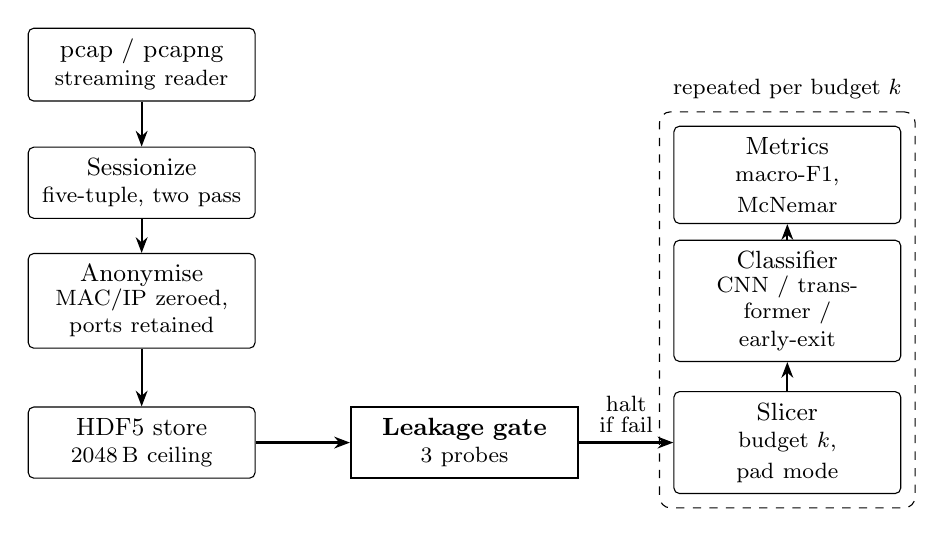
\begin{tikzpicture}[
  font=\small,
  box/.style={draw, rounded corners=2pt, align=center, inner sep=4pt,
              minimum height=9mm, text width=26mm},
  gate/.style={draw, thick, align=center, inner sep=4pt,
               minimum height=9mm, text width=26mm},
  ar/.style={-{Stealth[length=2mm]}, thick}
]
%% Left column: stages that run once, before any budget is chosen.
\node[box] (pcap)  at (0,0)     {pcap / pcapng\\[-1pt] \footnotesize streaming reader};
\node[box] (sess)  at (0,-1.5)  {Sessionize\\[-1pt] \footnotesize five-tuple, two pass};
\node[box] (anon)  at (0,-3.0)  {Anonymise\\[-1pt] \footnotesize MAC/IP zeroed,\\[-1pt] \footnotesize ports retained};
\node[box] (store) at (0,-4.8)  {HDF5 store\\[-1pt] \footnotesize 2048\,B ceiling};
%% Bottom row: the halt condition sits between the store and the sweep.
\node[gate] (lkg)  at (4.1,-4.8) {\textbf{Leakage gate}\\[-1pt] \footnotesize 3 probes};
%% Right column: the per-budget loop.
\node[box] (slice) at (8.2,-4.8) {Slicer\\[-1pt] \footnotesize budget $k$, pad mode};
\node[box] (model) at (8.2,-3.0) {Classifier\\[-1pt] \footnotesize CNN / transformer /\\[-1pt] \footnotesize early-exit};
\node[box] (met)   at (8.2,-1.4) {Metrics\\[-1pt] \footnotesize macro-F1, McNemar};
\node[draw, dashed, rounded corners, fit=(slice)(model)(met), inner sep=5pt] (loop) {};
\node[font=\footnotesize, above=1pt of loop] {repeated per budget $k$};
\draw[ar] (pcap)  -- (sess);
\draw[ar] (sess)  -- (anon);
\draw[ar] (anon)  -- (store);
\draw[ar] (store) -- (lkg);
\draw[ar] (lkg)   -- node[above, font=\footnotesize, align=center]
                        {halt\\[-2pt] if fail} (slice);
\draw[ar] (slice) -- (model);
\draw[ar] (model) -- (met);
\end{tikzpicture}
\caption{The measurement pipeline. Capture parsing, sessionization and
anonymisation run once; only the dashed region repeats per budget, so the
budget is the sole variable along a sweep. The leakage gate is a halt
condition, not a reported metric.}\label{fig:arch}
\end{figure}

\subsection{Anonymisation and the leakage gate}

MAC and IP bytes are zeroed in place, preserving offsets so that the budget
still means the same thing. Ports are deliberately \emph{retained}, because
discarding them would hide a shortcut rather than measure it. Three probes are
then trained on byte positions alone:

\begin{itemize}
\item $\textsc{id\_positions}$ reads the identifier byte positions from the
\emph{anonymised} store. This is the \textbf{gate}: it must not beat the
majority-class rate. If it does, anonymisation failed and no downstream number
is reported.
\item $\textsc{ident}$ reads the same positions \emph{before} anonymisation. A
high score is expected and quantifies how much identifier signal was destroyed.
\item $\textsc{ports}$ reads the retained port bytes. This is a reported risk,
not a gate.
\end{itemize}

\subsection{Padding modes}

To separate the input encoding from the padding symbol, four modes are defined
over the same slice:
\textsc{zero} (scalar $b/255$, zero padded, the byte-image baseline encoding);
\textsc{embed} (learned embedding of 256 byte values, ordinary zero padding);
\textsc{mask} (learned embedding over 257 symbols including an explicit
\textsc{pad}); and \textsc{convmask} (as \textsc{mask}, with padded positions
excluded from pooling using the true length). Comparing \textsc{zero} with
\textsc{mask} changes two things at once, which is what the literature does.
The attribution is therefore
\begin{align}
\Delta_{\text{repr}} &= \mathcal{F}_1(\textsc{embed}) - \mathcal{F}_1(\textsc{zero}),
\label{eq:drepr}\\
\Delta_{\textsc{pad}} &= \mathcal{F}_1(\textsc{mask}) - \mathcal{F}_1(\textsc{embed}),
\label{eq:dpad}
\end{align}
so that $\Delta_{\text{repr}} + \Delta_{\textsc{pad}}$ recovers the combined
effect while each term is separately interpretable. A fifth control,
\textsc{length\_balanced}, resamples the test set so that every retained class
spans the same flow-length bins, removing length as a cue.

\subsection{Causal early-exit classifier}

Reading fewer bytes only saves anything if the model can stop early. One
encoder is therefore trained with exits at depths
$\mathcal{E} = \{64, 128, 256, 512, 1024\}$ bytes. For head $k \in
\mathcal{E}$ to report an honest cost, its output must depend only on the first
$k$ bytes. Standard normalisation breaks this: batch and group normalisation
compute statistics across the length axis, so byte 900 shifts the activation at
position 10. The encoder therefore uses dilated \emph{causal} convolutions with
per-position channel normalisation,
\begin{equation}
\begin{aligned}
\mathrm{ChannelNorm}(h)_{c,t} &= \gamma_c \,
\frac{h_{c,t} - \mu_t}{\sqrt{\sigma_t^2 + \epsilon}} + \beta_c, \\
\mu_t &= \tfrac{1}{D}\textstyle\sum_{c} h_{c,t}, \\
\sigma_t^2 &= \tfrac{1}{D}\textstyle\sum_{c} (h_{c,t} - \mu_t)^2,
\end{aligned}
\label{eq:cnorm}
\end{equation}
where $D$ is the channel count, written separately from the class count $C$,
$\gamma_c$ and $\beta_c$ are learned per channel and $\epsilon$ guards the
square root. This normalises across channels
at each position $t$ and never mixes
positions. With receptive field confined to $[1,t]$ by causal padding, head $k$
provably returns identical logits from a truncated and a full input; a unit
test asserts bit-identical outputs.

Training minimises the mean cross-entropy over reachable heads,
\begin{equation}
\mathcal{L}(\theta) = \frac{1}{|\mathcal{E}_r|}
\sum_{k \in \mathcal{E}_r} \;
\mathbb{E}_{(s,y)} \big[\, \mathrm{CE}\big(f^{(k)}_\theta(x_k(s)),\, y \big) \big],
\label{eq:loss}
\end{equation}
where $\mathcal{E}_r$ contains only exits the ceiling actually reaches.
At inference, Algorithm~\ref{alg:exit} halts at the first head whose softmax
confidence clears a threshold $\tau$, and charges the bytes that head actually
consumed.

\begin{algorithm}[tbp]
\caption{Confidence-thresholded early exit}\label{alg:exit}
\begin{algorithmic}[1]
\Require session bytes $\mathbf{b}$, true length $L$, exits $\mathcal{E}$
(ascending), threshold $\tau$
\Ensure predicted class $\hat{y}$, bytes read $r$
\For{$k \in \mathcal{E}$}
  \State $p \gets \mathrm{softmax}\big(f^{(k)}_\theta(x_k(\mathbf{b}))\big)$
  \State $r \gets \min(k, L)$ \Comment{a short flow cannot cost more than it has}
  \If{$\max_c p_c \ge \tau$ \textbf{or} $k = \max \mathcal{E}$}
     \State \Return $\arg\max_c p_c,\; r$
  \EndIf
\EndFor
\end{algorithmic}
\end{algorithm}

Crucially, the policy is evaluated against \emph{the same model's own
fixed-depth heads}, not against a separate sweep. Comparing against the sweep
would confound the exit policy with differences in ceiling and representation.

\subsection{Changes from the original design}\label{sec:changes}

The methodology above departs from this project's original Phase~2 design in
five respects, each forced by something found while implementing or running
it rather than by preference, and each recorded here because it affects how
the results should be read.

\begin{enumerate}
\item \textbf{The input representation became a swept variable.} The original
design fixed bytes to a scalar in $[0,1]$. That encoding cannot separate
adjacent byte values, which differ by $0.004$ after scaling, and on synthetic
data with a cue past byte 780 it plateaus at $0.492$ macro-F1 where a learned
embedding reaches $1.000$. Because the budget curve is the study's instrument
and its shape depends on this choice, both encodings are swept
(Table~\ref{tab:padding}).
\item \textbf{The padding control gained an attribution arm.} Comparing zero
padding against a masked embedding changes two things at once, so the
\textsc{embed} mode was added to separate them by
Eqs.~\eqref{eq:drepr}--\eqref{eq:dpad}.
\item \textbf{The leakage control became three probes.} ``Train on the fields
that were anonymised'' is ambiguous, so it was split into the gate, the
context probe and the retained-field probe of
Section~\ref{sec:method}.
\item \textbf{The encoder was made causal.} The original design specified
early-exit heads at byte depths but not how to guarantee that a head sees only
the bytes it is charged for. Without that guarantee the accuracy-per-byte
frontier is meaningless, hence Eq.~\eqref{eq:cnorm}.
\item \textbf{The split strategy became an experiment.} The original design
treated the group-wise/temporal fallback as a caveat. Because it is the
study's largest confound, it was measured instead
(Section~\ref{subsec:fairness}).
\end{enumerate}

%%=========================================================================
\section{Experimental setup}\label{sec:setup}

\subsection{Datasets}

Two public corpora are used, chosen because the reviewed literature reports on
both. \textbf{USTC-TFC2016}~\cite{ustc} yields 353{,}496 sessions over ten
benign application classes and ten malware families, with a median true length
of 474 bytes; 1 of its 20 classes admits a group-wise split and 19 take the
temporal fallback. \textbf{ISCX VPN-nonVPN}~\cite{iscx} yields 31{,}855
sessions over 11 traffic categories captured with and without a VPN tunnel,
median length 274 bytes, with 6 of 11 classes group-splittable.

The ISCX release used here carries 140 capture files covering 11 of the 12
categories defined by the scheme: the non-VPN \texttt{p2p} captures are absent.
This was verified to be a property of the release rather than an incomplete
download by reading the five distributed archives directly: all 140 declared
captures are present and extracted, and the only \texttt{p2p} capture anywhere
in the distribution is the VPN one, which is already a separate class.
Studies reporting the full 12-class taxonomy are therefore working from a
different release or labelling, which is itself a comparability obstacle.


\subsection{Preprocessing and splits}

A streaming reader parses pcap and pcapng without loading captures into
memory. Sessions are assembled in two passes over each capture, keyed by
normalised five-tuple; sessions shorter than two packets are dropped and
byte-identical duplicates removed. Of the 140 ISCX captures only 101
contributed a unique session, because sessionizing by five-tuple merges
conversations the corpus ships split across \texttt{a} and \texttt{b} files.

The split is 70/15/15 and \emph{group-wise where the corpus allows it}: whole
capture files are held out, so test sessions come from captures never seen in
training. A class whose sessions come from fewer than three capture files
cannot be split that way, and falls back to a temporal split on first-packet
timestamp. As Section~\ref{sec:setup} notes, 19 of 20 USTC classes and 5 of 11
ISCX classes take the fallback. This is a property of the corpora, not a
choice, and Section~\ref{sec:results} measures what it is worth.

\subsection{Baselines}

Three published models are reimplemented and run at their own stated budgets:
the 2D byte-image CNN of Wang et al.~\cite{ustc} at 784 bytes, a 1D
byte-sequence CNN at 784 bytes, and Deep Packet at 1500 bytes. A byte-level
transformer is additionally implemented to test whether the budget response
depends on model family (Section~\ref{sec:results}).

\subsection{Metrics and statistical protocol}

The study reports accuracy, macro-F1, weighted-F1 and per-class
precision/recall/F1/support. Macro-F1 is primary because both corpora are
imbalanced and Gap 2 concerns minority classes. Every configuration is run with
seeds $\{0,1,2\}$ and reported as mean $\pm$ standard deviation; the
split-strategy study uses eight seeds.

Two tests are applied, because each alone misleads. The \textbf{seed-noise
rule} declares a difference inconclusive when it falls inside
$\sigma_{\text{seed}}$. \textbf{McNemar's exact test}~\cite{mcnemar} is applied
to the two genuinely paired comparisons, where the same test sessions are
scored by two models. Following Dietterich~\cite{dietterich}, McNemar is
appropriate only for paired predictions, so it is not used for comparisons
across seeds or corpora.

\subsection{Implementation details}

Models are implemented in PyTorch 2.11.0+cu130~\cite{pytorch} and trained on a
single NVIDIA RTX 5050 (8\,GB). The session store uses HDF5 via h5py
3.16.0~\cite{hdf5}. Optimiser Adam, learning rate $10^{-3}$, batch size 128
with automatic back-off on out-of-memory, cross-entropy loss, 40 epochs on
USTC and 15 on ISCX, which is capped at 5000 sessions per class. The causal
encoder follows the dilated-convolution design of WaveNet~\cite{wavenet}. All
code, configuration and result JSON are available
(Section~\ref{sec:declarations}).

%%=========================================================================
\section{Results and analysis}\label{sec:results}

\subsection{Leakage gate}

The gate passed on both corpora. On USTC the
$\textsc{id\_positions}$ probe reaches $0.1351 \pm 0.0014$ accuracy against a
majority-class rate of $0.1359$, i.e.\ $-0.0008$ excess over chance; on ISCX it
reaches $0.1095$ against $0.2258$, i.e.\ $-0.1164$. Anonymisation therefore
left no usable identifier signal. The context probes confirm there was signal
to destroy: $\textsc{ident}$, reading the same positions before anonymisation,
reaches $0.3851$ on USTC and $0.5330$ on ISCX, exceeding chance by $+0.2491$
and $+0.3071$. The $\textsc{ports}$ probe exceeds chance by $+0.6150$ on USTC
and $+0.0760$ on ISCX. Ports are thus a strong standalone predictor on USTC,
which Section~\ref{sec:ablation} shows the full model nonetheless barely uses.

\subsection{Baseline performance}

Table~\ref{tab:baselines} reports the three baselines at their own budgets. The
two corpora sit in different regimes: USTC is near ceiling, ISCX is hard. The
gap between accuracy and macro-F1 on ISCX (0.4419 against 0.5245 for the 1D
CNN) is itself informative, and is examined in Section~\ref{sec:discussion}.

\begin{table}[tbp]
\caption{Baselines at their own published budgets, mean $\pm$ s.d.\ over three
seeds. Macro-F1 is the primary metric.}\label{tab:baselines}
\begin{tabular}{@{}llrrr@{}}
\toprule
Corpus & Model & Budget & Accuracy & Macro-F1 \\
\midrule
\multirow{3}{*}{USTC-TFC2016}
 & 2D byte image~\cite{ustc} & 784 B & $0.9566 \pm 0.0245$ & $0.9595 \pm 0.0095$ \\
 & 1D byte sequence & 784 B & $0.9407 \pm 0.0154$ & $0.9564 \pm 0.0018$ \\
 & Deep Packet & 1500 B & $0.9460 \pm 0.0206$ & $0.9574 \pm 0.0045$ \\
\midrule
\multirow{3}{*}{ISCX VPN-nonVPN}
 & 2D byte image~\cite{ustc} & 784 B & $0.4523 \pm 0.0326$ & $0.5108 \pm 0.0099$ \\
 & 1D byte sequence & 784 B & $0.4419 \pm 0.0265$ & $0.5245 \pm 0.0208$ \\
 & Deep Packet & 1500 B & $0.4327 \pm 0.0545$ & $0.5018 \pm 0.0258$ \\
\botrule
\end{tabular}
\end{table}

\subsection{Per-class behaviour (Gap 2)}\label{sec:perclass}

Table~\ref{tab:perclass} gives the per-class breakdown on ISCX at 784 bytes,
from the uncapped stratified run so that the class distribution is the
corpus's own. Two things are visible here that no aggregate reports.

\textbf{The direction of the concealment reverses between corpora.} On ISCX
macro-F1 is 0.5110 against a weighted-F1 of 0.3798, so the macro average
\emph{flatters} the model by 13 points; on USTC macro-F1 is 0.9245 against a
weighted-F1 of 0.9378, so it \emph{understates} by 1 point. A reader who
assumes a fixed relationship between the two summaries is wrong about the sign
on one of the two corpora, which is the concrete form Gap 2 takes.

\textbf{Two failure modes are invisible in the aggregate.} \texttt{vpn\_chat}
is the second-largest class in the test set, 686 of 4047 sessions, and the
model assigns it a recall of 0.042: it almost never predicts the class, though
when it does it is usually right (precision 0.744). Its mirror image is
\texttt{vpn\_file}, which attains a recall of 1.000 at a precision of 0.241 and
is acting as a sink for sessions the model cannot place. Neither is a thin
class scraping by on low support, and neither is discernible in an accuracy of
0.4013.

\begin{table}[tbp]
\caption{Per-class results on ISCX VPN-nonVPN at a 784-byte budget, uncapped
run, ordered by support. The aggregate is accuracy 0.4013, macro-F1 0.5110,
weighted-F1 0.3798 over 4047 test sessions.}\label{tab:perclass}
\begin{tabular}{@{}lrrrr@{}}
\toprule
Class & Support & Prec. & Recall & F1 \\
\midrule
\texttt{chat}          & 914 & 0.474 & 0.580 & 0.522 \\
\texttt{vpn\_chat}     & 686 & 0.744 & \textbf{0.042} & \textbf{0.080} \\
\texttt{voip}          & 593 & 0.398 & 0.290 & 0.336 \\
\texttt{streaming}     & 474 & 0.684 & 0.643 & 0.663 \\
\texttt{vpn\_voip}     & 443 & 0.125 & 0.174 & 0.145 \\
\texttt{email}         & 417 & 0.172 & 0.177 & 0.175 \\
\texttt{vpn\_file}     & 149 & \textbf{0.241} & \textbf{1.000} & 0.389 \\
\texttt{file}          & 145 & 0.899 & 0.676 & 0.772 \\
\texttt{vpn\_streaming}& 110 & 0.716 & 0.755 & 0.735 \\
\texttt{vpn\_p2p}      &  72 & 0.844 & 0.903 & 0.872 \\
\texttt{vpn\_email}    &  44 & 0.913 & 0.955 & 0.933 \\
\botrule
\end{tabular}
\end{table}

\subsection{The budget response (Gap 1)}

Table~\ref{tab:budget} and Figure~\ref{fig:budget} give the central result.
Macro-F1 saturates at 512 bytes on USTC and 256 bytes on ISCX by
Eq.~\eqref{eq:sat}. On the packet axis, saturation falls at 5 packets on USTC
and 2 packets on ISCX.

\begin{table}[tbp]
\caption{Byte-budget response, macro-F1 (mean $\pm$ s.d., three seeds), with
the mean padding fraction $\mathbb{E}[\rho_k]$ from Eq.~\eqref{eq:rho} beside
each budget. Saturation points by Eq.~\eqref{eq:sat} in bold; budgets used by
reviewed studies marked.}\label{tab:budget}
\begin{tabular}{@{}lrrrrl@{}}
\toprule
& \multicolumn{2}{c}{USTC-TFC2016} & \multicolumn{2}{c}{ISCX VPN-nonVPN} & \\
\cmidrule(lr){2-3}\cmidrule(lr){4-5}
Budget & Macro-F1 & $\mathbb{E}[\rho_k]$ & Macro-F1 & $\mathbb{E}[\rho_k]$ & Used by \\
\midrule
64 B   & $0.9188 \pm 0.0047$ & 0.000 & $0.4643 \pm 0.0158$ & 0.002 & \\
128 B  & $0.9426 \pm 0.0070$ & 0.006 & $0.5031 \pm 0.0212$ & 0.021 & \\
256 B  & $0.9652 \pm 0.0041$ & 0.105 & $\mathbf{0.5061 \pm 0.0191}$ & 0.244 & \\
512 B  & $\mathbf{0.9731 \pm 0.0006}$ & 0.242 & $0.5078 \pm 0.0096$ & 0.478 & \\
784 B  & $0.9564 \pm 0.0018$ & 0.307 & $0.5245 \pm 0.0208$ & 0.587 & \cite{ustc,p10} \\
1024 B & $0.9540 \pm 0.0118$ & 0.347 & $0.5092 \pm 0.0326$ & 0.639 & \cite{p8} \\
1500 B & $0.9367 \pm 0.0142$ & 0.398 & $0.5083 \pm 0.0288$ & 0.701 & \\
\midrule
$\sigma_{\text{seed}}$ & \multicolumn{2}{c}{0.0142} & \multicolumn{2}{c}{0.0326} & \\
\botrule
\end{tabular}
\end{table}

\begin{figure}[tbp]
\centering
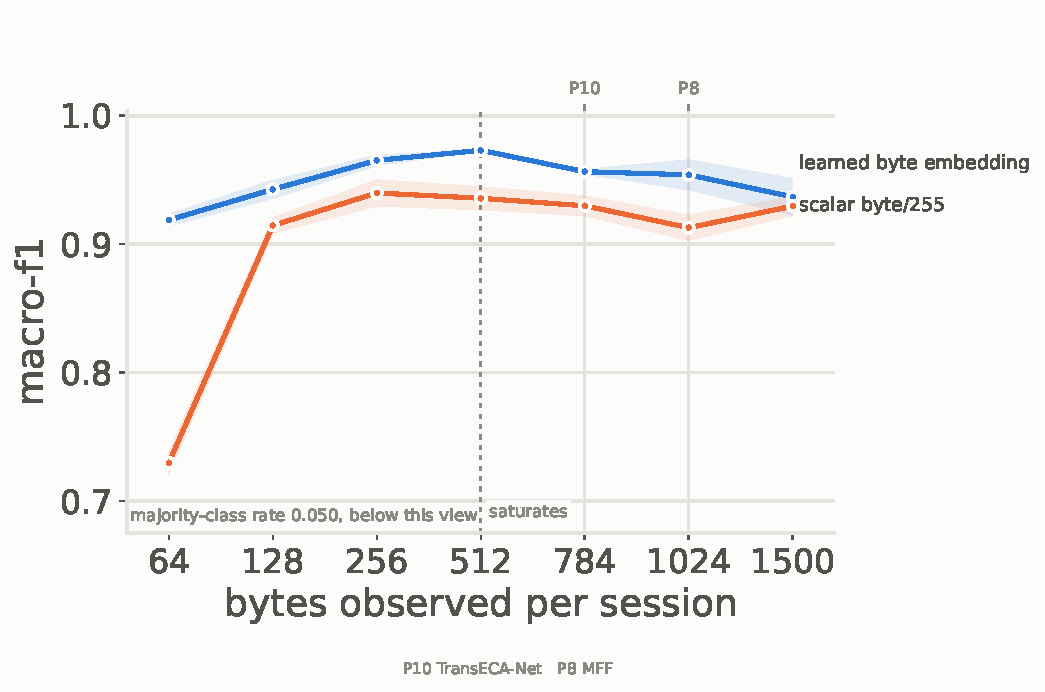
\includegraphics[width=0.49\textwidth]{figures/ustc_budget_profile_bytes.pdf}
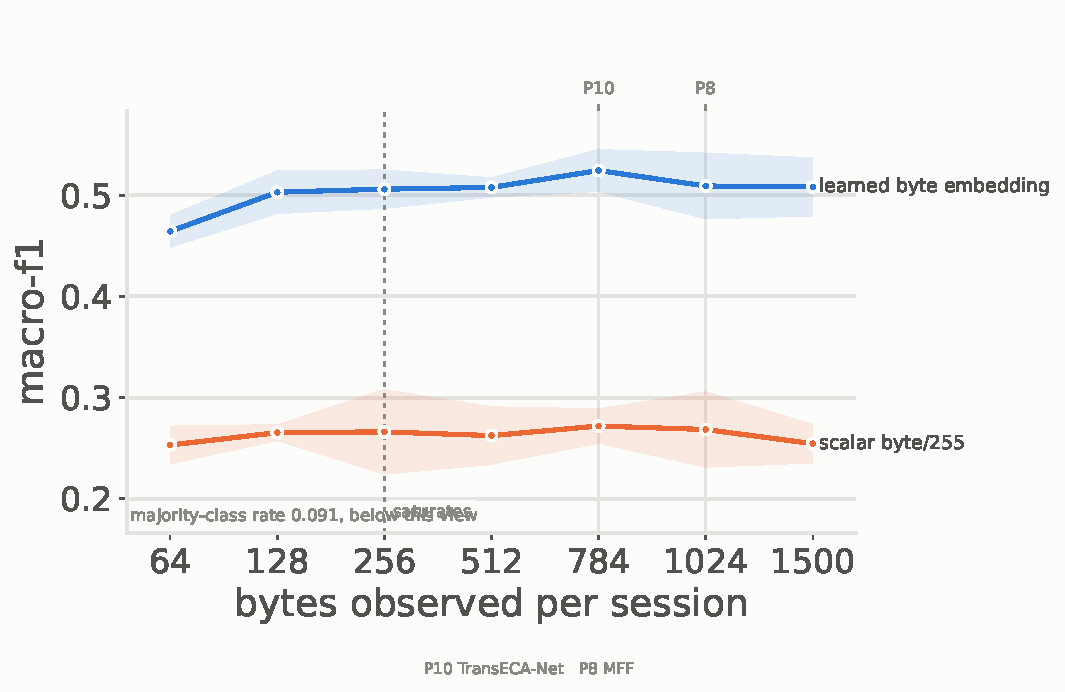
\includegraphics[width=0.49\textwidth]{figures/iscx_budget_profile_bytes.pdf}
\caption{Byte-budget response on USTC-TFC2016 (left) and ISCX VPN-nonVPN
(right). Shaded bands are seed spread; vertical marks are budgets used by the
reviewed studies. Every marked budget lies at or past the saturation
point.}\label{fig:budget}
\end{figure}

Three observations follow.

\textbf{Every reviewed budget lies at or past saturation.} The budgets in the
literature are 784 and 1024 bytes, and 5, 15, 16 and 20 packets. On both
corpora all of them sit at or beyond $k^\star$. The gain available past
saturation is $-0.0167$ on USTC and $+0.0184$ on ISCX, against seed noise of
$0.0142$ and $0.0326$ respectively: on ISCX the remaining gain is smaller than
the noise, and on USTC it is negative.

\textbf{On USTC, reading further actively hurts.} Macro-F1 falls from 0.9731 at
512 bytes to 0.9367 at 1500 bytes. This is the one comparison where the paired
test is decisive. McNemar's test at seed 0 on 51{,}963 test sessions gives
$n_{10} = 2488$ sessions correct at 512 bytes but wrong at 784, against
$n_{01} = 94$ in the other direction, $p < 10^{-4}$
(Table~\ref{tab:mcnemar}). Reading 1.53$\times$ more bytes does not merely stop
helping; it costs accuracy, and reliably so.

\textbf{The harder corpus saturates earlier.} ISCX saturates at 256 bytes
against USTC's 512. This is the opposite of the intuition that a harder problem
needs more evidence, and it is consistent with the padding explanation: at 256
bytes ISCX is already 24.4\% padding, and at 784 bytes it is 58.7\%.

\begin{table}[tbp]
\caption{McNemar's exact test~\cite{mcnemar} on the two paired comparisons,
seed 0. $n_{10}$ counts sessions where A is correct and B is not.}\label{tab:mcnemar}
\begin{tabular}{@{}llrrrl@{}}
\toprule
Corpus & Comparison (A vs B) & $n_{10}$ & $n_{01}$ & $p$ & Reading \\
\midrule
USTC & 512 B vs 784 B & 2488 & 94 & $<10^{-4}$ & A better \\
USTC & ports kept vs masked & 2277 & 107 & $<10^{-4}$ & A better \\
ISCX & 256 B vs 784 B & 174 & 254 & $1.3\times10^{-4}$ & B better \\
ISCX & ports kept vs masked & 234 & 217 & $0.451$ & no difference \\
\botrule
\end{tabular}
\end{table}

The two tests disagree on ISCX, and that is reported rather than resolved by
choosing between them: McNemar finds 784 bytes significantly better than 256
($p = 1.3\times10^{-4}$) while the seed rule finds the same $+0.0184$
inconclusive against $\sigma_{\text{seed}} = 0.0326$. Both are correct, because
McNemar asks whether a difference is reproducible on \emph{these} sessions at
\emph{this} seed and the seed rule asks whether it survives retraining. A
difference that is highly significant under McNemar yet vanishes across seeds
is one a practitioner cannot rely on, which is a reason for caution about any
single-seed significance claim in this literature.

\subsection{Padding attribution (Gap 1, continued)}

Table~\ref{tab:padding} decomposes the padding control by
Eqs.~\eqref{eq:drepr}--\eqref{eq:dpad}. On ISCX, moving from the scalar
\textsc{zero} encoding to a learned embedding is worth $+0.2408$ macro-F1,
while adding an explicit \textsc{pad} symbol on top of that is worth $+0.0086$,
well inside seed noise of $0.0373$. The gain routinely credited to
``padding-aware'' input is therefore almost entirely the input representation,
not the padding treatment. On USTC both terms ($+0.0138$ and $+0.0065$) fall
inside seed noise of $0.0176$, so that corpus supports neither attribution, and it
is reported as the null result it is, and the claim rests on ISCX alone.
Figure~\ref{fig:padding} in Appendix~\ref{app:extra} plots both
decompositions against their seed-noise bands.

\begin{table}[tbp]
\caption{Padding control at a 1024-byte budget, macro-F1. The attribution
splits the usual \textsc{zero}-to-\textsc{mask} comparison into a
representation term and a padding-symbol term.}\label{tab:padding}
\begin{tabular}{@{}lrr@{}}
\toprule
Mode & USTC-TFC2016 & ISCX VPN-nonVPN \\
\midrule
\textsc{zero} (scalar $b/255$) & $0.9351 \pm 0.0067$ & $0.2684 \pm 0.0373$ \\
\textsc{embed} (learned, zero pad) & $0.9489 \pm 0.0069$ & $0.5092 \pm 0.0326$ \\
\textsc{mask} (learned + \textsc{pad}) & $0.9553 \pm 0.0176$ & $0.5178 \pm 0.0183$ \\
\textsc{convmask} (masked pooling) & $0.9399 \pm 0.0053$ & $0.3001 \pm 0.0235$ \\
\midrule
$\Delta_{\text{repr}}$ (Eq.~\ref{eq:drepr}) & $+0.0138$ & $\mathbf{+0.2408}$ \\
$\Delta_{\textsc{pad}}$ (Eq.~\ref{eq:dpad}) & $+0.0065$ & $+0.0086$ \\
$\sigma_{\text{seed}}$ & $0.0176$ & $0.0373$ \\
Conclusive? & neither term & representation only \\
\botrule
\end{tabular}
\end{table}


\subsection{Accuracy per byte read}

Figure~\ref{fig:frontier} reports the early-exit policy against the same
model's own fixed-depth heads, with the head-by-head breakdown as
Table~\ref{tab:frontier} in Appendix~\ref{app:extra}. On USTC the policy
matches the best fixed head (0.9716 macro-F1 at 512 bytes) while reading 144
bytes on average, \textbf{28\% of the byte cost}. On ISCX it matches the best
head (0.5474 at 512 bytes) at 116 bytes, \textbf{23\% of the cost}. Because the
encoder is causal by Eq.~\eqref{eq:cnorm}, these byte counts are real: head $k$
cannot have seen byte $k+1$. The positive control for the whole instrument,
run on generated traffic with a planted cue, is in Appendix~\ref{app:synth}.


\begin{figure}[tbp]
\centering
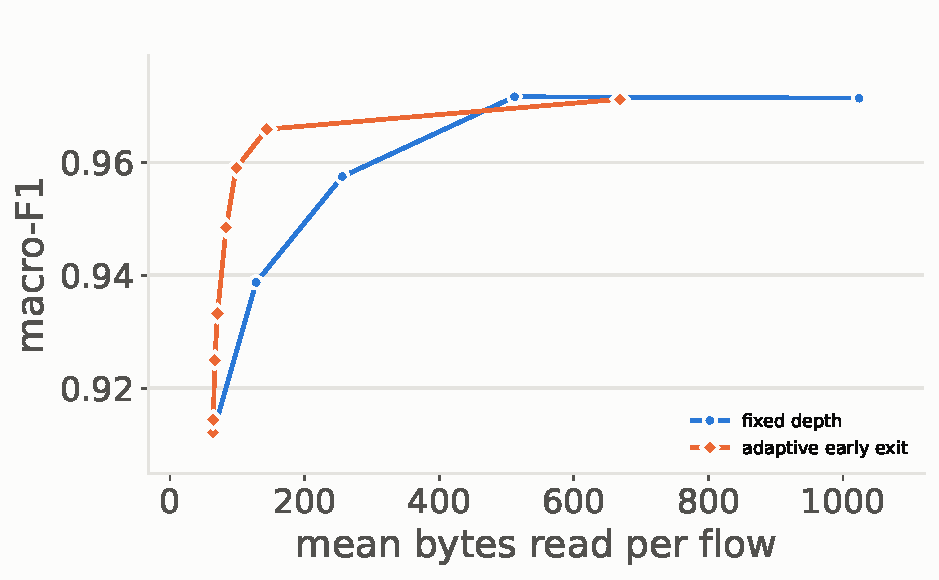
\includegraphics[width=0.49\textwidth]{figures/ustc_accuracy_per_byte_frontier.pdf}
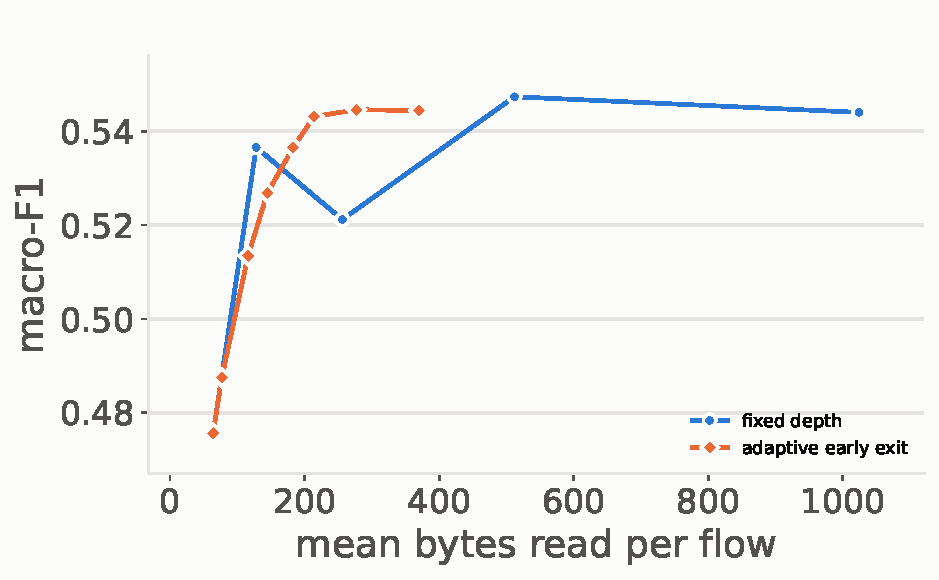
\includegraphics[width=0.49\textwidth]{figures/iscx_accuracy_per_byte_frontier.pdf}
\caption{Accuracy-per-byte frontier on USTC (left) and ISCX (right). Fixed
budgets against the adaptive early-exit policy; the policy reaches the best
fixed head's macro-F1 at a fraction of the byte cost.}\label{fig:frontier}
\end{figure}

\subsection{Architecture independence}

Every baseline above is a convolutional network from 2017--2020, whereas all
twelve reviewed studies use transformers or graph networks. If the saturation
point were an artefact of convolution, the finding would not transfer. The
whole sweep was therefore repeated on ISCX with a byte-level transformer
(patch tokenisation by strided convolution, four pre-norm encoder layers, four
heads, key-padding mask) on the same store, split manifest, schedule and seeds.

The two families are not separable: peak macro-F1 is $0.5245 \pm 0.0208$ for
the CNN and $0.5195 \pm 0.0379$ for the transformer, a difference of $-0.0050$
that lies inside the seed spread of both. Packet saturation falls at 2 packets
under both. On the byte axis they differ nominally (256 B against 128 B), but
the gain each leaves past its own saturation point ($+0.0184$ and $+0.0176$) is
smaller than its own seed noise ($0.0326$ and $0.0399$): they agree saturation
is early and disagree only about which early budget. The budget response is
thus a property of where discriminative bytes lie, not of the network reading
them. This transformer is trained from scratch and its absolute scores are
\emph{not} comparable to pre-trained models~\cite{p6,p7}; only the shape of the
curve is.

%%=========================================================================
\section{Comparison with base papers and state of the art}\label{sec:basepapers}

\subsection{Summary of the base papers}

The base papers are those this work is built on: the byte-image formulation of
Wang et al.~\cite{ustc}, which supplies the 784-byte budget and the 2D
baseline; P10~\cite{p10} and P8~\cite{p8}, which carry the 784- and 1024-byte
budgets into 2025; P7~\cite{p7}, which states that its budget was fixed by a
token ceiling; and P5~\cite{p5}, whose occlusion study motivates the leakage
gate. Table~\ref{tab:basepapers} summarises them.

\begin{table}[tbp]
\caption{Base papers: problem, method, data, metrics, reported results and the
limitation this work responds to. Values marked $*$ are taken from the original
publication under its own protocol; every unmarked number anywhere in this
paper was produced by the authors' own runs.}\label{tab:basepapers}
\small
\begin{tabular}{@{}p{13mm}p{17mm}p{17mm}p{16mm}p{14mm}p{26mm}@{}}
\toprule
Paper & Problem & Method & Dataset & Reported & Key limitation \\
\midrule
Wang et al.\ 2017~\cite{ustc} &
Malware / app ID &
2D byte image + CNN &
USTC (20 cls) &
Acc 0.998* &
Budget fixed by $28\times28$ image shape, not measured \\
\addlinespace
P10 2025~\cite{p10} &
Encrypted app ID &
Transformer + channel attention &
ISCX (12 cls), USTC (10 cls) &
Acc 0.9765*, 0.9825* &
Inherits 784 B; per-class far below headline (VoIP 92.20\%) \\
\addlinespace
P8 2025~\cite{p8} &
Encrypted app ID &
Multimodal feature fusion &
ISCX (12 cls), USTC (20 cls) &
Acc 0.9961*, 0.9999* &
1024 B pads $\approx$87\% of ISCX sessions; no macro-F1 \\
\addlinespace
P7 2025~\cite{p7} &
Encrypted app ID &
Multi-level pre-training &
ISCX (6 cls), USTC (20 cls) &
F1 0.9880*, 0.9926* &
Budget set by 512-token ceiling by authors' own account \\
\addlinespace
P5 2025~\cite{p5} &
Evaluating classifiers &
Field occlusion study &
ISCX &
Acc 0.96$\to$0.51* &
Shows the shortcut but does not gate pipelines on it \\
\botrule
\end{tabular}
\end{table}

\subsection{Quantitative comparison}

Table~\ref{tab:quant} places this study's results beside the base papers on
the same corpora. It should be stated plainly that \textbf{this work does not outperform the base
papers on headline accuracy}, and that the comparison is not like-for-like.
The differences are quantified rather than asserted in
Section~\ref{subsec:fairness}.

\begin{table}[tbp]
\caption{Quantitative comparison. Starred rows are figures reported by the
original authors under their own protocol; unstarred rows are this study's runs under
the protocol of Section~\ref{sec:setup}. ``Bytes'' is the observation budget
actually consumed.}\label{tab:quant}
\begin{tabular}{@{}llrrrl@{}}
\toprule
Corpus & Method & Classes & Bytes & Acc / F1 & Split \\
\midrule
\multirow{5}{*}{USTC}
 & P8 MFF* ~\cite{p8}            & 20 & 1024 & 0.9999 acc & not stated \\
 & P7 MLETC* ~\cite{p7}          & 20 & 500  & 0.9926 F1  & not stated \\
 & P10 TransECA* ~\cite{p10}     & 10 & 784  & 0.9825 acc & not stated \\
 & Ours, best fixed budget       & 20 & 512  & 0.9731 F1  & group/temporal \\
 & \textbf{Ours, adaptive}       & 20 & \textbf{144} & \textbf{0.9716 F1} & group/temporal \\
\midrule
\multirow{5}{*}{ISCX}
 & P8 MFF* ~\cite{p8}            & 12 & 1024 & 0.9961 acc & not stated \\
 & P4 MH-Net* ~\cite{p4}         & 6  & 15 pkt & 0.9941 F1 & not stated \\
 & P10 TransECA* ~\cite{p10}     & 12 & 784  & 0.9765 acc & not stated \\
 & P5 (ET-BERT, IDs removed)* ~\cite{p5} & -- & varies & 0.5100 acc & not stated \\
 & \textbf{Ours, adaptive}       & 11 & \textbf{116} & \textbf{0.5474 F1} & group/temporal \\
\botrule
\end{tabular}
\end{table}

\subsection{Methodological comparison}

Three differences separate this work from the base papers, each addressing a
stated limitation.

\textbf{The budget is measured, not inherited.} Where Wang et al., P10 and P8
fix a budget by input shape or convention, this study sweeps 64--2048 bytes
and 1--20 packets from one store and reports the curve with seed variance, which is what
makes it possible to say their budgets sit past saturation.

\textbf{Padding is decomposed rather than mitigated.} The base papers report
the combined benefit of a padding-aware representation; splitting it by
Eqs.~\eqref{eq:drepr}--\eqref{eq:dpad} shows it lives in the embedding, not the
padding symbol. A practitioner reading those papers would conclude that
handling \textsc{pad} explicitly matters. It does not; switching from scalar to
embedded bytes does.

\textbf{Leakage is a halt condition, not a discussion point.} P5 demonstrates
the identifier shortcut; here it becomes a gate that stops the pipeline, with
the port probe reported beside every headline number.

\subsection{Improvement analysis}

The improvement this work offers is in observation cost, not accuracy. Against
the 784-byte budget of Wang et al.\ and P10, the adaptive policy reads 144
bytes on USTC, an absolute reduction of 640 bytes and a relative reduction of
\textbf{81.6\%}; against P8's 1024 bytes the reduction is \textbf{85.9\%}. On
ISCX the 116-byte policy is \textbf{85.2\%} below 784 bytes and
\textbf{88.7\%} below 1024. These savings come from two sources that the
measurements separate: most sessions are classified correctly by an early head
(the budget response is flat past $k^\star$), and the remaining budget is
increasingly padding rather than content (Table~\ref{tab:budget}).

On accuracy this study is below the base papers on both corpora: 2.0 points of
macro-F1 below P7's reported USTC figure (0.9731 against 0.9926), and far below
on ISCX. This is not attributed
to the models being better or worse, because the protocols differ in ways
Section~\ref{subsec:fairness} quantifies.

\subsection{Fairness and limitations of the comparison}\label{subsec:fairness}

Four differences prevent a fair comparison, and the largest of them was
measured rather than conceded.

\textbf{Split policy, worth $+0.3782$ macro-F1.} None of the base papers states
how its train/test boundary was formed. On the six ISCX classes with enough
capture files to be split either way, holding the classes, budget, model,
epochs, seeds \emph{and per-class split sizes} fixed and varying only the
boundary gives Table~\ref{tab:split}, plotted as Figure~\ref{fig:split} in
Appendix~\ref{app:extra}: a random within-capture split scores
$0.9378$ macro-F1 where a group-wise split scores $0.5596$. The difference,
$+0.3782$, is 7.4 times the seed noise and larger than every architectural
effect measured in this paper combined. An accuracy near 0.94 on this corpus is
reachable without the model generalising past the capture file at all. This
does not prove the base papers used a random split, but it establishes that the
gap between these numbers and theirs is within the range that split policy
alone can explain.

\begin{table}[tbp]
\caption{Split-strategy study on ISCX, six group-splittable classes, eight
seeds, 256-byte budget, 14{,}697 training and 2{,}275 test sessions in every
arm, chance rate 0.1667.}\label{tab:split}
\begin{tabular}{@{}lrrl@{}}
\toprule
Train/test boundary & Accuracy & Macro-F1 & vs group-wise \\
\midrule
Group-wise (unseen captures) & $0.5388 \pm 0.0431$ & $0.5596 \pm 0.0510$ & reference \\
Temporal (same captures, later) & $0.6439 \pm 0.0337$ & $0.6027 \pm 0.0337$ & $+0.0431$ (inconclusive) \\
Random (same captures) & $0.9463 \pm 0.0038$ & $0.9378 \pm 0.0046$ & $\mathbf{+0.3782}$ (inflated) \\
\botrule
\end{tabular}
\end{table}


\textbf{Class scheme.} The ISCX runs here use 11 classes because the release
contains 11 (Section~\ref{sec:setup}). P4 and P7 report on 6, P8 and P10 on 12.
A 6-class problem is not the same problem.

\textbf{Identifier fields.} The gate used here guarantees identifier bytes
are unlearnable. P9 retains source and destination addresses as explicit
inputs~\cite{p9}, and P1 and P2 do not state their treatment. P5 measures this
shortcut at up to 0.45 accuracy~\cite{p5}, which is of the same order as the
gap between the ISCX numbers here and theirs. The closest like-for-like figure in
the literature is P5's ET-BERT with identifiers removed, 0.51 accuracy, which
is in the same regime as the results reported here.

\textbf{Pre-training.} P6 and P7 pre-train on large unlabelled corpora. The
models here, including the transformer, are trained from scratch on the target
corpus. Absolute scores are therefore not compared against them, and no such
claim is made.

%%=========================================================================
\section{Ablation study}\label{sec:ablation}

Table~\ref{tab:ablation} reports four ablations plus the port and length
controls. Verdicts use the seed-noise rule; null results are reported as null.

\begin{table}[tbp]
\caption{Ablations, macro-F1 (mean $\pm$ s.d., three seeds). A difference
inside $\sigma_{\text{seed}}$ is reported as inconclusive rather than as a
small effect.}\label{tab:ablation}
\footnotesize
\begin{tabular}{@{}p{18mm}p{32mm}r r p{18mm}@{}}
\toprule
Ablation & Variant & USTC & ISCX & Verdict \\
\midrule
\multirow{3}{18mm}{Representation}
 & 1D sequence (ref., 106k par.) & $0.9564 \pm 0.0018$ & $0.5245 \pm 0.0208$ & reference \\
 & 2D byte image (3.3M par.) & $0.9595 \pm 0.0095$ & $0.5108 \pm 0.0099$ & inconclusive \\
 & Deep Packet (324k par.) & $0.9615 \pm 0.0209$ & $0.5064 \pm 0.0050$ & inconclusive \\
\midrule
\multirow{3}{18mm}{Layer scope}
 & All layers (reference) & $0.9564 \pm 0.0018$ & $0.5245 \pm 0.0208$ & reference \\
 & Headers only & $0.9531 \pm 0.0083$ & $0.4857 \pm 0.0635$ & inconclusive \\
 & Payload only & $0.9018 \pm 0.0012$ & $0.4268 \pm 0.0039$ & \textbf{worse} \\
\midrule
\multirow{2}{18mm}{Granularity}
 & Bidirectional session (ref.) & $0.9500 \pm 0.0304$ & $0.5234 \pm 0.0275$ & reference \\
 & Unidirectional flow & $0.9545 \pm 0.0131$ & $0.4259 \pm 0.0111$ & session better (ISCX) \\
\midrule
\multirow{2}{18mm}{Early-exit supervision}
 & All heads supervised (ref.) & $0.9714 \pm 0.0129$ & $0.5440 \pm 0.0383$ & reference \\
 & Terminal head only & $0.9794 \pm 0.0074$ & $0.5338 \pm 0.0162$ & inconclusive \\
\midrule
Port control & Largest macro-F1 lost to masking & $-0.0428$ & $-0.0040$ & see text \\
Length control & Flow length equalised & $0.7907 \pm 0.0133$ & $0.1106 \pm 0.0319$ & see text \\
 & (chance within balanced set) & $0.1429$ & $0.1667$ & \\
\botrule
\end{tabular}
\end{table}

\textbf{Representation contributes nothing at matched budget.} All three
baselines fall within seed noise of each other on both corpora, despite a
31-fold spread in parameter count (106k to 3.3M). The 2D byte image, which
motivated the 784-byte budget, buys nothing over a 1D sequence once the budget
is held fixed. This matters for Gap 1: the budget is inherited from an
architecture whose advantage is not reproducible here.

\textbf{Payload-only input is clearly worse, headers-only is not.} Restricting
to payload costs 0.055 macro-F1 on USTC and 0.098 on ISCX, both outside noise.
Restricting to headers costs nothing measurable. Combined with the budget
curve, this locates the discriminative bytes in the early header region, which
is why saturation arrives so early.

\textbf{Granularity disagrees across corpora, for a nameable reason.} On
ISCX the bidirectional session beats the unidirectional flow by 0.098, outside
noise. On USTC the difference ($+0.0045$) is inside noise and inconclusive. The
ISCX result must be read with care: splitting sessions into directional flows
lowers the median true length from 274 to 159 bytes, so the flow setting is the
more truncated one, and this design cannot separate a granularity effect from a
truncation effect.

\textbf{Early-exit supervision is not free but is not costly.} Supervising all
heads rather than only the terminal head changes macro-F1 by $-0.0080$ on USTC
and $+0.0102$ on ISCX, both inside noise. The multi-head loss of
Eq.~\eqref{eq:loss} therefore buys the early-exit capability at no measurable
accuracy cost, which is the result that makes Table~\ref{tab:frontier}
worth having.

\textbf{Ports are available but unused.} The $\textsc{ports}$ probe exceeds
chance by $+0.6150$ on USTC, yet masking the port bytes costs the full model
only $0.0428$ macro-F1 there and $0.0040$ on ISCX. McNemar finds the USTC
masking effect significant and the ISCX one not ($p = 0.451$,
Table~\ref{tab:mcnemar}). The shortcut exists and is redundantly encoded: the
model does not depend on it.

\textbf{Length is a large part of the ISCX signal.} With flow length equalised
across classes, USTC holds $0.7907$ macro-F1 against a chance rate of $0.1429$,
while ISCX falls to $0.1106$ against $0.1667$, i.e.\ to chance. Content still
separates USTC's classes with length held fixed; on ISCX it barely does. The
control retains only 168 and 84 test sessions respectively and a biased subset
of classes, so the direction is reported and the magnitude declined.

%%=========================================================================
\section{Discussion}\label{sec:discussion}

\subsection{Why the budget response behaves this way}

Three measurements point to one mechanism. The layer-scope ablation locates the
discriminative bytes in the header region; the budget curve saturates early;
and the padding fraction at those budgets is already 0.24 on both corpora.
Past saturation the marginal byte is therefore increasingly \textsc{pad} rather
than content, and on USTC accuracy then \emph{falls} significantly, consistent
with padding acting as noise the model must learn to ignore with no
compensating signal.

\subsection{Practical implications}

The result is directly actionable: a system reading 1024 bytes per flow to
replicate P8's budget pays 7.1$\times$ the byte cost of the adaptive policy for
accuracy the budget curve says is not there. Reading less also shortens
detection latency and reduces per-flow memory, both of which matter on a
middlebox.

\subsection{Strengths}

The study's strength is control: every budget is a slice of one store, so no
sweep point differs in sessionization, deduplication or class balance;
causality is proved rather than assumed, so ``bytes read'' is a real cost; and
every claim carries seed variance, with an exact test on the two paired
comparisons.

\subsection{Limitations and failure cases}\label{subsec:limits}

\begin{enumerate}
\item \textbf{Split strategy is confounded with corpus difficulty.} 19 of 20
USTC and 5 of 11 ISCX classes take the temporal fallback, and the corpus that
scores higher is also the one split the easier way, so no comparison
\emph{between} corpora separates difficulty from split policy.
Table~\ref{tab:split} measures the policy \emph{within} ISCX and finds the
temporal fallback indistinguishable from group-wise ($+0.0431$ against
$\sigma_{\text{seed}} = 0.0510$), so the headline numbers here are not inflated the
way a random split's would be; the cross-corpus comparison still is.
\item \textbf{The length-balanced control is underpowered}, leaving 168 and 84
test sessions and a biased class subset: direction reportable, magnitude not.
\item \textbf{Encryption strata are bounds.} The TLS tagger leaves part of each
corpus unresolved, so Gap 3 is answered as a lower bound: under 8\% of either
corpus is \emph{confirmed} encrypted, less than ``encrypted-traffic benchmark''
implies. P5's 95--99\% estimate~\cite{p5} is neither reproduced nor
contradicted.
\item \textbf{The ISCX class list is short by one} and its per-application
labels are heuristic, so the category scheme is used throughout.
\item \textbf{The transformer is trained from scratch} on a schedule tuned for
convolutional networks. Its curve shape is comparable; its heights are not
comparable to pre-trained models.
\item \textbf{Failure case.} The clearest failure is ISCX \texttt{vpn\_chat}
in Table~\ref{tab:perclass}, at 0.042 recall on 686 test sessions, with
\texttt{vpn\_file} absorbing the misplaced traffic at 0.241 precision.
\end{enumerate}

\subsection{Threats to validity}

\emph{Internal:} three seeds is a small variance sample, which is why the split
study uses eight, and single-seed significance can disagree with the seed rule.
\emph{External:} both corpora are 2016 laboratory captures, so the cipher mix
is dated and the saturation budget may differ on modern traffic.
\emph{Construct:} macro-F1 on 11 or 20 classes is not the construct that
6-class macro-F1 measures.

\subsection{Were the gaps and objectives met?}

\textbf{Gap 1 is answered}: saturation is measured at 512 and 256 bytes, every
reviewed budget sits at or past it, and on USTC reading further is
significantly worse. \textbf{Gap 2 is answered} by
Table~\ref{tab:perclass}: the macro/weighted gap reverses sign between corpora
and \texttt{vpn\_chat} sits at 0.042 recall inside a 0.4013 aggregate. \textbf{Gap 3 is partially answered}, as a lower bound
only. \textbf{Gap 4 is answered}: the gate passed on both corpora and the port
shortcut is available but unused.

%%=========================================================================
\section{Conclusion and future work}\label{sec:conclusion}

This paper treated the observation budget of raw-byte encrypted traffic
classification as a quantity to be measured rather than inherited. Macro-F1
saturates at 512 bytes on USTC-TFC2016 and 256 bytes on ISCX VPN-nonVPN, every
budget used by twelve recent studies lies at or past that point, and on USTC
reading further is significantly worse under McNemar's test. The gain usually
credited to padding-aware input comes almost entirely from the learned byte
embedding rather than the padding symbol. A causal early-exit classifier
matches the best fixed-depth head while reading 28\% and 23\% of the bytes.
Finally, a random within-capture split is worth $+0.3782$ macro-F1 on otherwise
identical data, exceeding every architectural effect measured here.

Future work follows from the limitations. A corpus in which more classes can be
split group-wise would let split policy be varied without the class-selection
bias of Table~\ref{tab:split}. A larger length-balanced subset, or a different
way of holding length fixed, would turn the directional finding of
Section~\ref{sec:ablation} into a magnitude. Pre-training the byte transformer
on unlabelled captures would test whether the saturation point moves once the
representation is learned rather than fitted. Finally, repeating the sweep on
contemporary traffic with a modern cipher mix would establish whether a
512-byte saturation point is a property of these 2016 captures or of encrypted
traffic generally.

%%=========================================================================


%%=========================================================================
\section*{Declarations}\label{sec:declarations}
\addcontentsline{toc}{section}{Declarations}

\textbf{Data availability.} Both corpora are public. USTC-TFC2016 is available
from its authors~\cite{ustc}; ISCX VPN-nonVPN is distributed by the Canadian
Institute for Cybersecurity~\cite{iscx}. No new data were collected.

\textbf{Code availability.} The complete implementation, configuration files
and the result JSON behind every table and figure in this paper are held in a
single repository, which will be released publicly on publication and is
available from the corresponding author in the interim. Figures and tables are
generated from that JSON by script; none is transcribed by hand.

\textbf{Reproducibility.} Random seeds are $\{0,1,2\}$ for all experiments and
$\{0,\dots,7\}$ for the split-strategy study. Hyperparameters, hardware and
software versions are given in Section~\ref{sec:setup}. The preprocessing
ceiling is 2048 bytes; ISCX runs are capped at 5000 sessions per class. Five
verification scripts run on generated captures and require no corpus, including
one that plants a cue at a known byte depth and requires the sweep to recover
it.

\textbf{Competing interests.} The authors declare no competing interests.

\textbf{Funding.} No funding was received for this work.

\textbf{Use of AI-assisted tools.} The authors used an AI assistant (Anthropic
Claude) during this project and declare its use as follows. The project
documentation, and the drafting and copy-editing of this manuscript, were
produced with AI assistance. For the experimental pipeline and the other major
components of the work, AI assistance was used in part, while the research
design, the implementation decisions, the experimental runs and the
verification of every reported result were carried out by the authors, who
performed the majority of the work. All experiments were run on the authors'
own hardware, and every unstarred number in this paper comes from those runs.
The authors have reviewed the entire manuscript and take full responsibility
for its content.

\section*{Acknowledgements}

The authors thank the course instructor for guidance across the four phases of
this project.

%%=========================================================================

\begin{appendices}

\section{Validation on synthetic ground truth}\label{app:synth}

Before either corpus was touched, the pipeline was validated on generated
traffic with a known answer: a weak cue at byte 78 and a strong cue past byte
780. The sweep recovers the planted structure exactly, tracing chance at 64
bytes, 0.837 macro-F1 at 128 bytes and 1.000 at 1500 bytes, and the leakage
gate separates 1.000 before anonymisation from 0.125 after. The scalar
\textsc{zero} encoding plateaus at 0.492 and never finds the late cue, because
after scaling two adjacent byte values differ by 0.004. This is a positive
control for the instrument, not a result about real traffic.

\section{Supporting tables and figures}\label{app:extra}

\begin{table}[tbp]
\caption{Fixed-depth heads of the early-exit model, macro-F1, against the
adaptive policy. All heads come from one training run, so the only difference
is whether the exit policy runs.}\label{tab:frontier}
\begin{tabular}{@{}lrrrr@{}}
\toprule
& \multicolumn{2}{c}{USTC-TFC2016} & \multicolumn{2}{c}{ISCX VPN-nonVPN} \\
\cmidrule(lr){2-3}\cmidrule(lr){4-5}
Exit & Bytes & Macro-F1 & Bytes & Macro-F1 \\
\midrule
head@64 B   & 64   & $0.9121 \pm 0.0039$ & 64   & $0.4756 \pm 0.0383$ \\
head@128 B  & 128  & $0.9388 \pm 0.0136$ & 128  & $0.5366 \pm 0.0434$ \\
head@256 B  & 256  & $0.9575 \pm 0.0231$ & 256  & $0.5212 \pm 0.0505$ \\
head@512 B  & 512  & $0.9716 \pm 0.0124$ & 512  & $0.5474 \pm 0.0495$ \\
head@1024 B & 1024 & $0.9714 \pm 0.0129$ & 1024 & $0.5440 \pm 0.0383$ \\
\midrule
\textbf{Adaptive policy} & \textbf{144} & $\mathbf{0.9716}$ & \textbf{116} & $\mathbf{0.5474}$ \\
Fraction of best fixed cost & \textbf{28\%} & & \textbf{23\%} & \\
\botrule
\end{tabular}
\end{table}

\begin{figure}[tbp]
\centering
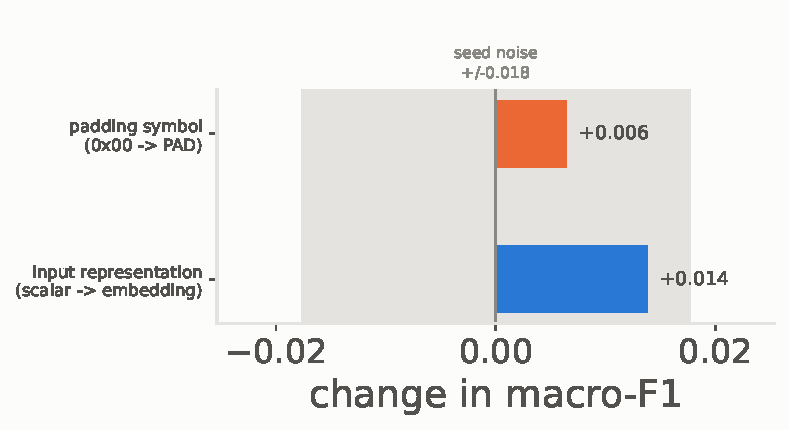
\includegraphics[width=0.49\textwidth]{figures/ustc_padding_attribution.pdf}
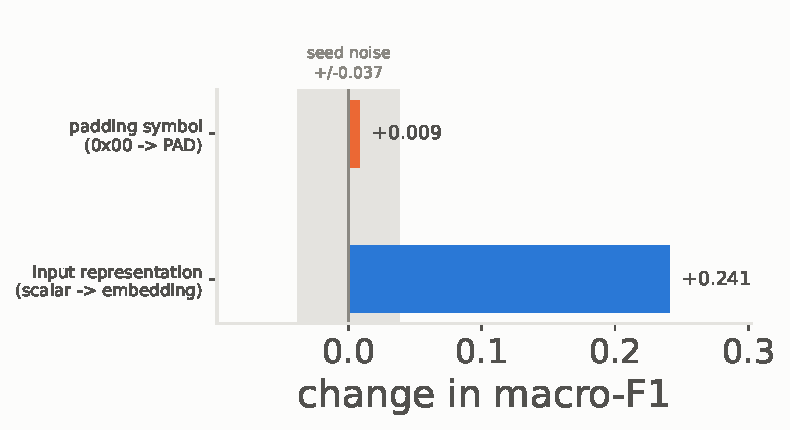
\includegraphics[width=0.49\textwidth]{figures/iscx_padding_attribution.pdf}
\caption{Padding attribution on USTC (left) and ISCX (right), against the
seed-noise band. On ISCX the representation term clears the band and the
padding-symbol term does not; on USTC neither does.}\label{fig:padding}
\end{figure}

\begin{figure}[tbp]
\centering
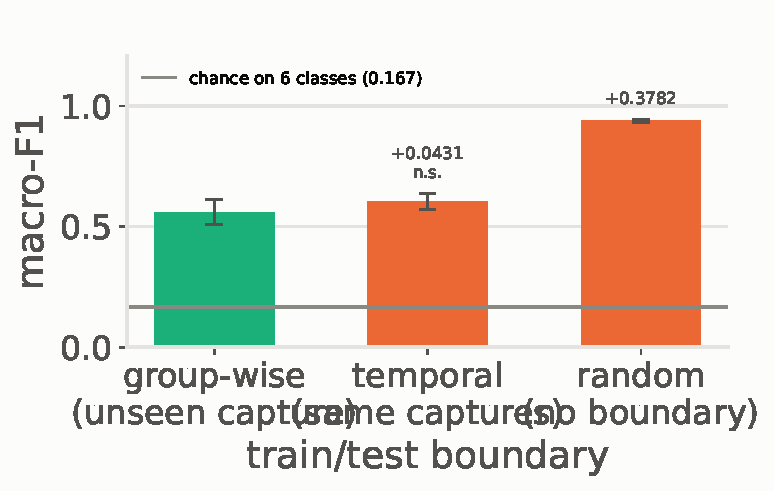
\includegraphics[width=\columnwidth]{figures/iscx_split_strategy.pdf}
\caption{Macro-F1 against where the train/test boundary falls, with classes,
budget, model, epochs, seeds and per-class split sizes held fixed. Error bars
are seed spread; the dashed line is the chance rate.}\label{fig:split}
\end{figure}

\end{appendices}

\bibliography{references}

\end{document}
